\documentclass{article}
\usepackage[utf8]{inputenc}
\usepackage{tikz}
\usetikzlibrary{shapes.geometric, arrows}
\tikzset{io/.style={
  trapezium, 
  trapezium left angle=70, 
  trapezium right angle=110, 
  text width=3cm, 
  minimum height=1cm, 
  text centered,
  draw=black, 
  fill=blue!30,
  trapezium stretches=true
  }}
  
\usepackage{adjustbox}  
\begin{document}
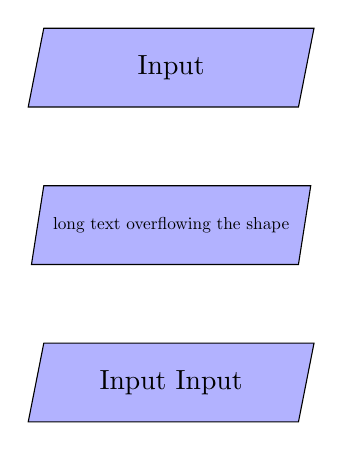
\begin{tikzpicture}[node distance=2cm]
\node (in1) [io] {Input};
\node at (0,-2) [io] {\adjustbox{max width=3cm}{long text overflowing the shape}};
\node at (0,-4) [io] {Input Input};
\end{tikzpicture}
\end{document}
